\documentclass[12pt]{article}
%\documentclass[12pt, letterpaper, twoside]{article}
\usepackage{graphicx}
\usepackage{xcolor}
\usepackage{subcaption}
\usepackage{hyperref}
\definecolor{linkcolour}{rgb}{0,0,1}
\hypersetup{colorlinks=true, urlcolor=linkcolour, linkcolor=linkcolour, linkbordercolor=linkcolour, pdfborderstyle={/S/U/W 1}} 
\urlstyle{same}

\usepackage{setspace} 
\singlespacing

\usepackage{geometry}
\geometry{margin=1in}

\setlength\parindent{0pt}

\graphicspath{{images/}}

\begin{document}
\title{Bike-Share Case Study}
\date{}
\maketitle

This report provides the results and step-by-step explanation of the data analysis performed for a bike-sharing case study. The data belongs to a bike-sharing company that has two kinds of users: annual members and casual riders. The goal of the study was to identify how annual members and casual riders use the bikes differently in order to help the stake-holders decide whether or not to target converting casual riders into annual members in the next marketing campaign. Python was used to perform the analysis using data collected from January-November 2023 and downloaded from \url{https://divvy-tripdata.s3.amazonaws.com/index.html}.

\section*{Cleaning:}
The code that was used to perform the data exploration can be found in the Jupyter Notebook \href{https://github.com/SummerKassem/BikeShareCS/blob/main/Code/cleaning.ipynb}{cleaning.ipynb}. The main functions are explained below:
\begin{itemize}
	\item \textit{read\_data}:\\
	Here the .csv file for the bike rides of each month are read and stored into a dictionary. Each element in the dictionary has a key (the name of the month) and a value (the Panada data-frame that holds the data entries). This simplifies the access of the entries for each corresponding month, by using the month as the key (e.g. original\_data[“May”] retrieves the data-frame that holds the entries from May), while maintaining the segregation between months (data from different months are not fused together). In Figure \ref{fig1} we can see the first and last 5 entries of bike rides from May:

	\begin{figure}[h]
	\hspace{-1.8cm}
	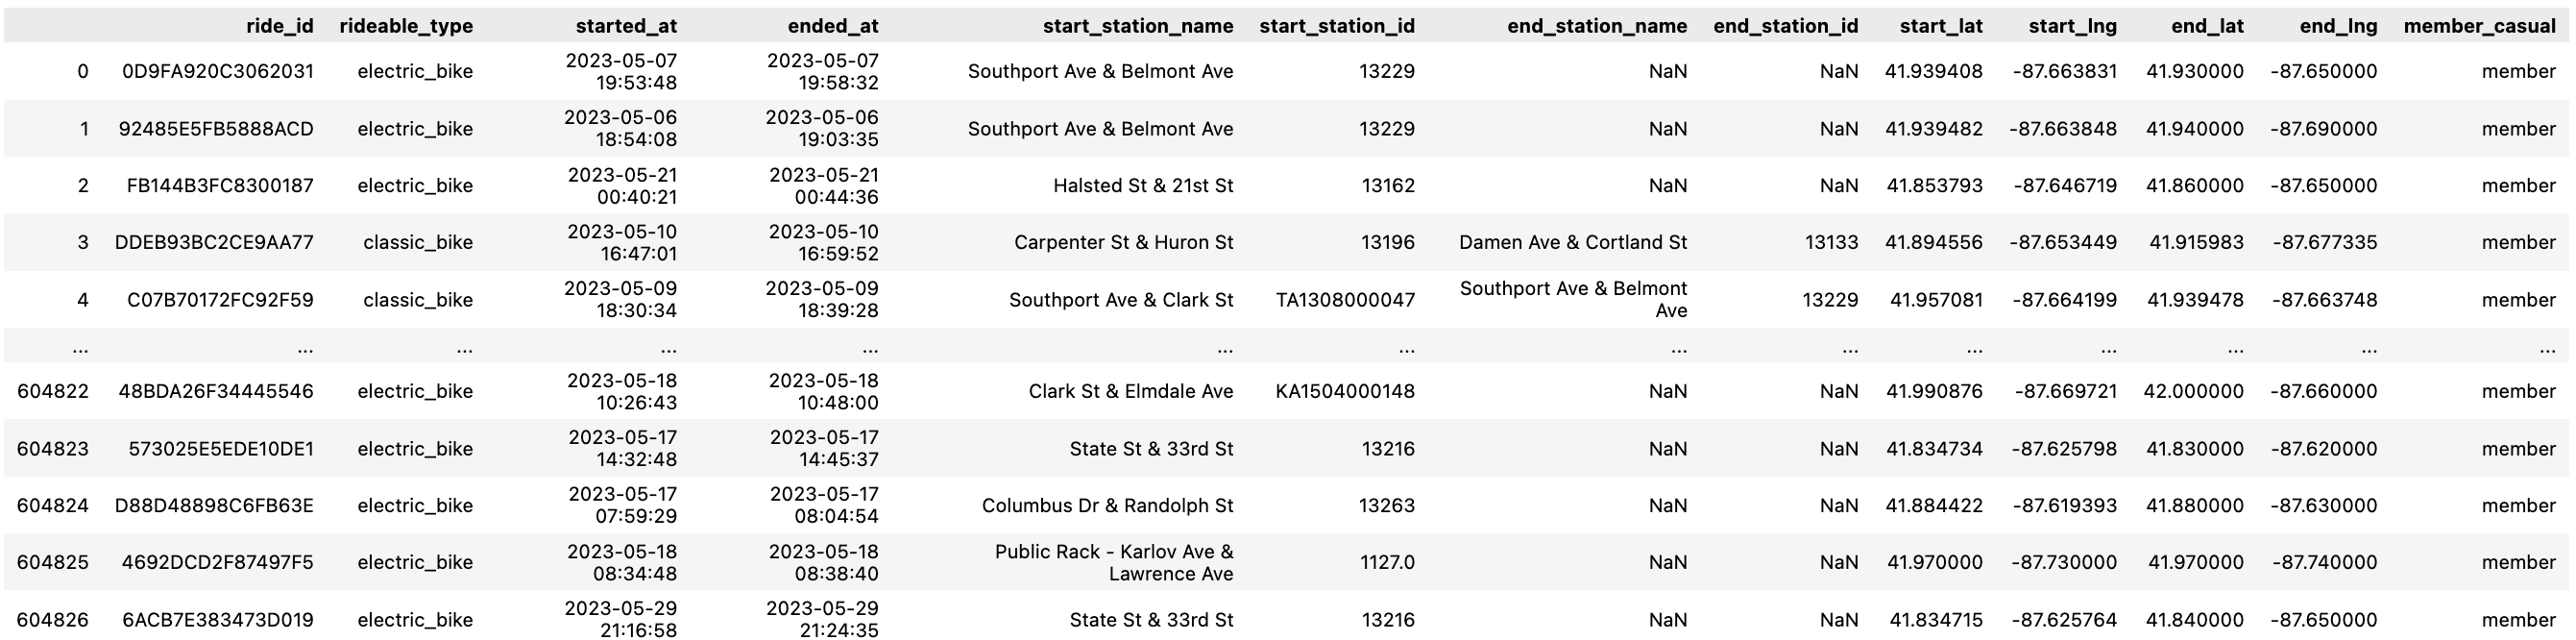
\includegraphics[width=8 in, height = 2 in]{imgMay.png}
	\caption{First and last 5 entries of bike rides from May (original\_data[``May"])}
	\label{fig1}
	\end{figure}
	\pagebreak
	
	From the entries we can see that the data consists of 13 columns: 1) ride id, 2) type of bike, 3-4) date and time for the start and end of the ride, 5-12) the name, id, latitude and longitude of the start and end stations, and 13) whether the rider was a casual rider or a member. 
	
	\item \textit{count\_entries}:\\
	After the csv files are read into the data-frames, the method \textit{count\_entries} is used to collect further information about the dataset. It finds the number of entries per file as well as the number of columns. This is done in order to check that the data format is consistent across the different files. Next, the method calculates the total number of bike rides in the entire dataset. There is an option within the method to remove duplicates. Therefore, the method is first called with the remove duplicates option deactivated, in order to collect preliminary information about the dataset. And then the method is called again with the remove duplicates option activated. The results are shown in Figure \ref{fig3}. 
	
	\begin{figure}[h]
	\centering
	\begin{subfigure}{.4\textwidth}
	\hspace{0.5 in}
		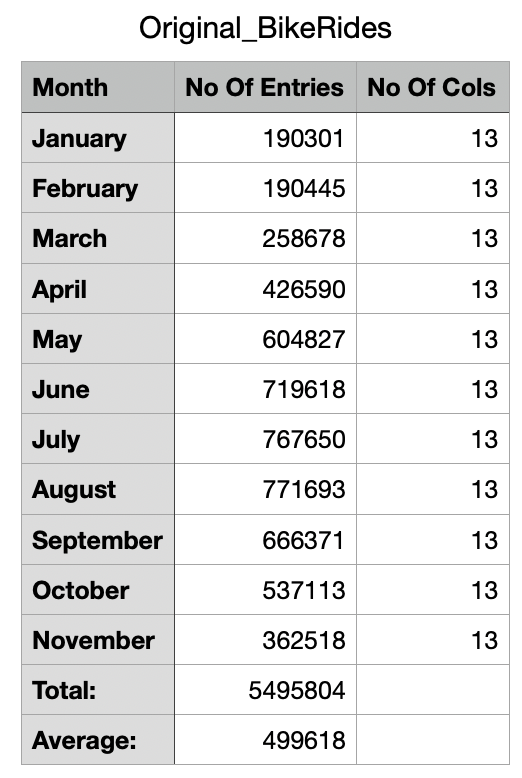
\includegraphics[scale=0.5]{img2.png}
	\end{subfigure}
	\begin{subfigure}{.4\textwidth}
	\hspace{0.5 in}
		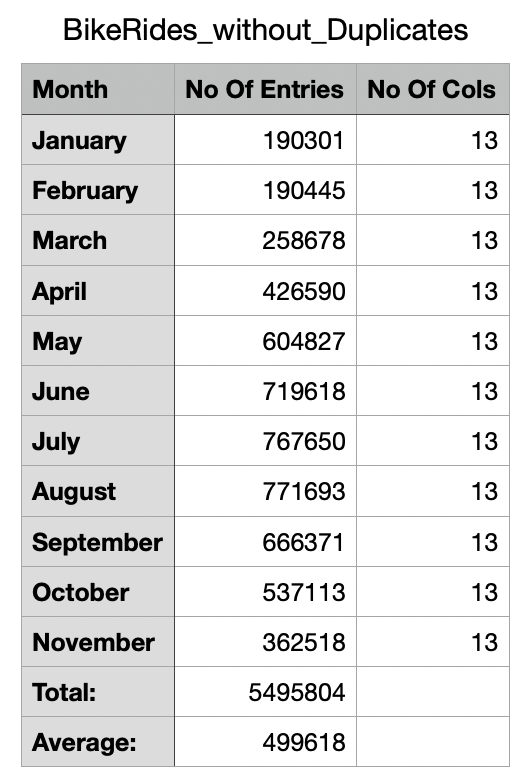
\includegraphics[scale=0.5]{img3.png}
	\end{subfigure}
	\caption{No of entries and columns before and after removing duplicates}
	\label{fig3}
	\end{figure}
	
The table in Figure \ref{fig3} on the left is the result of running the method without removing duplicates, and the table on the right is the result after removing duplicates. We can see that all the files have the same number of columns, which is a good preliminary indicator of the consistency of data across the months. In total the dataset contains almost 5.5 Million entries, with an average of approximately 500,000 entries per month. From January to March the number of rides is relatively lower than the average, which is expected as these are cold months. This is confirmed by the peak in the number of rides during the Summer months June to August. The number of entries before and after removing duplicates is identical, therefore the original dataset did not have any duplicates. \\

	\item \textit{check\_NAN}:\\
	Given that a brief look at the entries from May already showed a couple of NaN values (Figure \ref{fig1} \textit{end\_station\_name}, and \textit{end\_station\_id}), the method \textit{check\_NAN} calculates the percentage of NaN values for each column and month. The results are shown in Figure \ref{fig4}. As we can see the columns \textit{start\_station\_name}, \textit{start\_station\_id}, \textit{end\_station\_name}, \textit{end\_station\_id} in every month have 13-17\% null values. The columns \textit{end\_lat} and \textit{end\_long} have less than 1\% null values. 
	
	\begin{figure}[h]
	%\hspace{-1.8cm}
	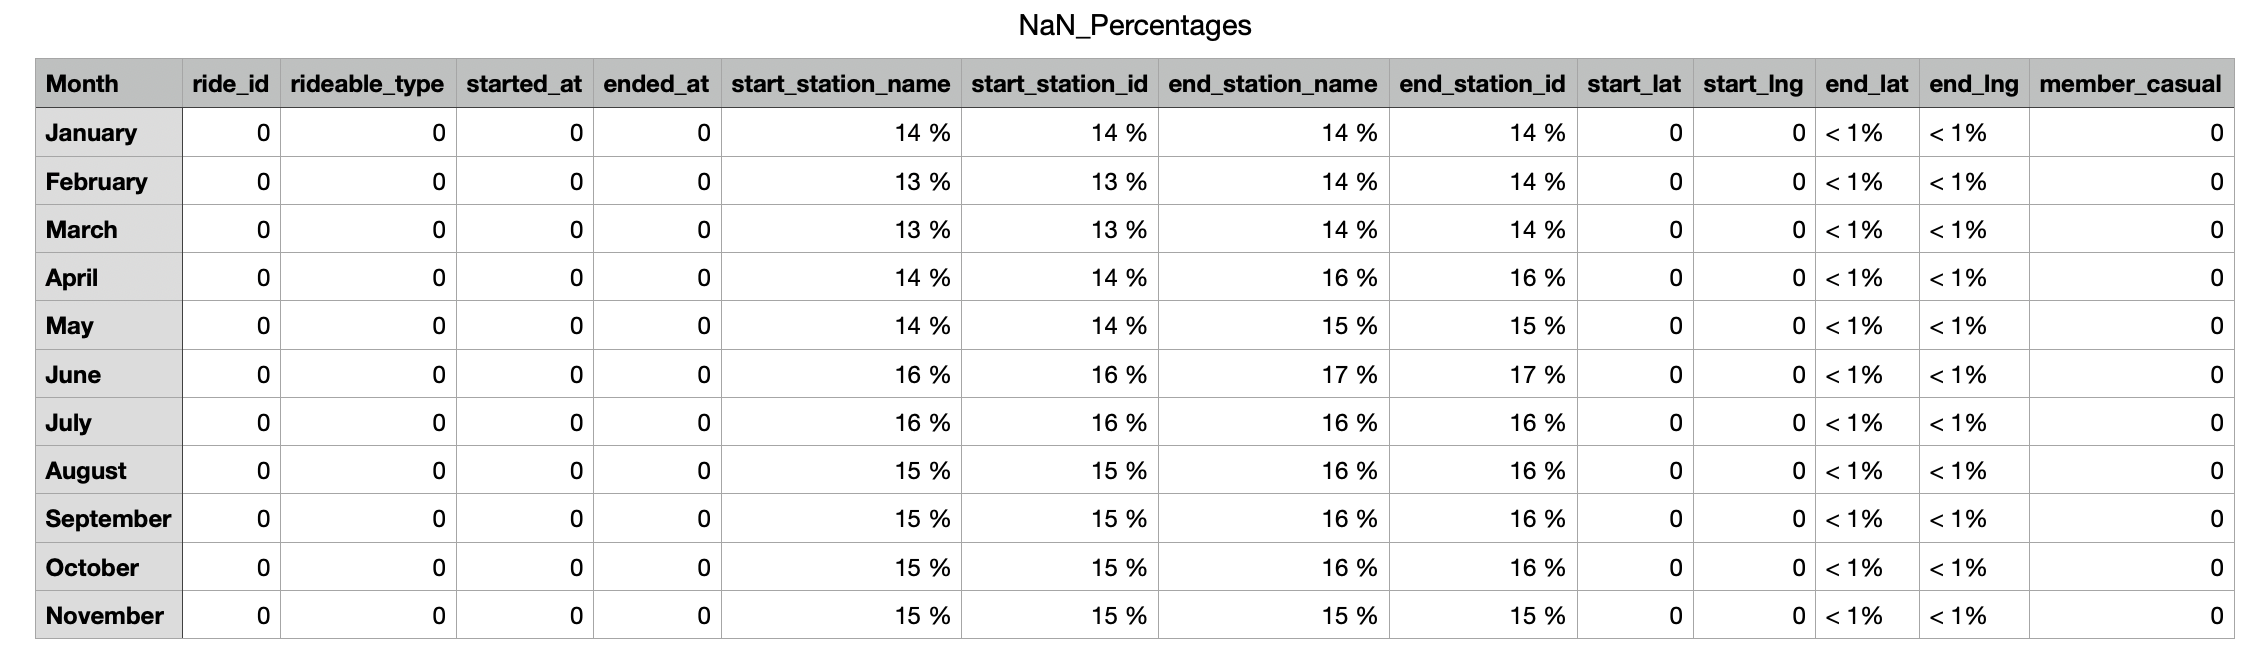
\includegraphics[width=6.5 in, height = 2.3 in]{imgNAN.png}
	\caption{Percentage of null values for each column across the various months}
	\label{fig4}
	\end{figure}
	
In order to explore the dataset a bit further, the number of unique (distinct) values for each column in original\_data[``May"] is calculated and shown in Figure \ref{fig2}. 
	\begin{figure}[h]
	\centering
	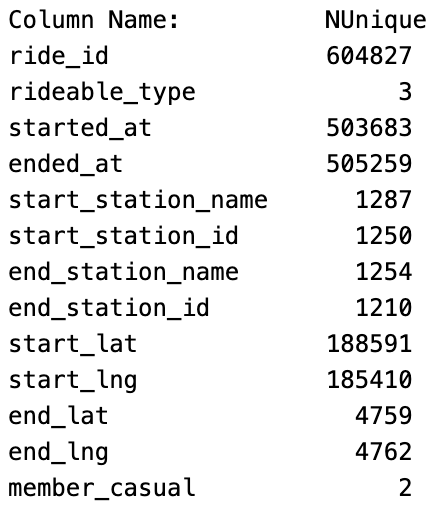
\includegraphics[scale = 0.6]{imgUnique.png} %[width=8 in, height = 2 in]
	\caption{No. of unique values for every column in original\_data[``May"]}
	\label{fig2}
	\end{figure}
	
\begin{itemize}
	\item \textit{ride\_id\_unique}  = 604827: as expected, has as many unique values as the number of entries in the dataframe.
	\item \textit{rideable\_type\_unique} = 3: these 3 unique values are:  [electric\_bike, classic\_bike, docked\_bike].
	\item \textit{started(ended)\_at\_unique} = 503683,  505259: since these are datetimes (yy-mm-dd hh:mm:ss), one may have expected that they would have as many distinct values as the number of entries, since it seems unlikely for more than one rider to have rented a bike at the exact same time down to the second. However, the number of unique values in these columns is less than the number of entries by 17\%. To ensure that these are not duplicate entries but with different \textit{ride\_id}, one of these incidents has been retrieved and is shown in Figure \ref{fig10}. By looking at the values, it is clear that they are indeed different entries but with the exact same start time.
	
	\begin{figure}[h]
	\hspace{-1.8cm}
	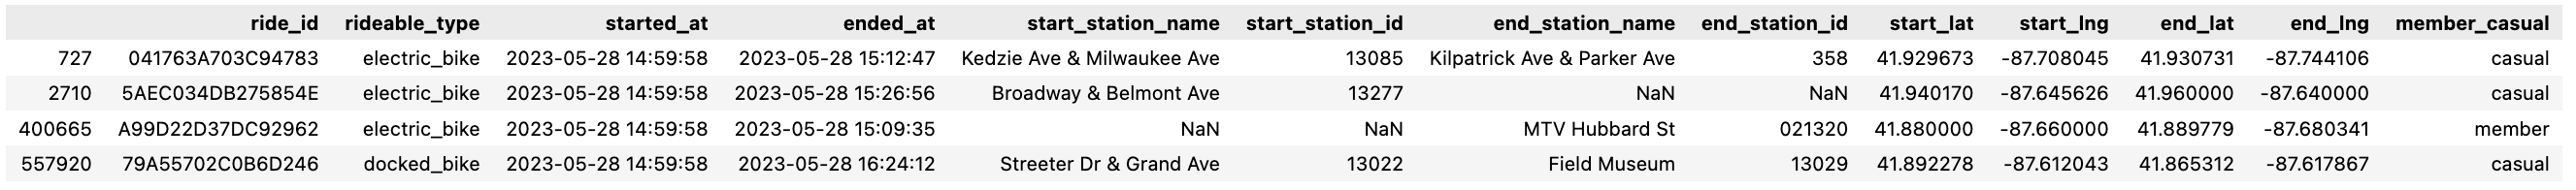
\includegraphics[width=8 in, height = 1 in]{imgDups1.png}
	\caption{Entries from original\_data[``May"] that have the exact same \textit{started\_at}}
	\label{fig10}
	\end{figure}
	
	\item \textit{start(end)\_station\_name(id)\_unique} = 1287, 1250, 1254, 1210: since there is a limited number of stations, it is expected that these columns have a smaller number of unique values than the number of entries. However, one would have expected the number of unique station names and station ids to be the same, whereas the ids are less than the names by a small fraction. Which could either by accounted for by the null values or could mean that there are stations that have the different names but the same id.
	\item \textit{start(end)\_lat(long)\_unique} = 188591, 185419, 4759, 4762: the start latitude and longitude numbers seem to be as expected, which is less than the total number of entries, but more than the number of stations (since the exact location where a bike is docked can vary within the station especially that the values are given to the $6^{th}$ decimal place). However, there is a large difference between the number of values in the start ($\sim$188000) and the numbers in the end ($\sim$4800) latitude and longitude. This difference cannot be accounted for by the null values in the end columns, since these were less than 1\%. If these values are true, that would mean that users rode there bikes from many start points, but ended up in a much smaller set of points. Which cannot be the case since that would have been reflected in the number of end stations. 
	\item \textit{member\_casual\_unique} = 2: these 2 unique values are: [member, casual].
\end{itemize}
	
	\item \textit{clean\_data}:\\
	After exploring the dataset, we can see that the extractable information can be divided into information about the:
	\begin{enumerate} 
	\item rider (casual/member)
	\item bike (electric/classic/docked)
	\item ride (start-end: time, date, location)
	\end{enumerate}
Since, the goal of the analysis is to find out whether to target converting casual riders into members or not, it seems that all the information is relevant to the analysis, with the exception of the ride location. The geographical location would have been important if for example the goal of the analysis was to find out whether more stations should be added and where to do so. Therefore, since the locations seem to be irrelevant, contain null values and discrepancies, these columns will be dropped. The column \textit{ride\_id} also does not provide any valuable information for the current analysis. Thus, the first task performed by the method \textit{clean\_data} is to drop all columns related to geographical location and ride id, which leaves: \textit{rideable\_type}, \textit{started\_at}, \textit{ended\_at}, \textit{member\_casual}. 


Next, is data formatting. We have already looked at the columns \textit{rideable\_type} and \textit{member\_casual}, and ensured that they have the expected values. As for the columns \textit{started\_at} and \textit{ended\_at}, we need to make sure that the \textit{ended\_at} time always comes after \textit{started\_at} time. In order to compare the values, they are first converted to a numerical datetime format, since they were stored as strings of characters. Next, by comparing the values and filtering them, we find that there are indeed cases where the \textit{ended\_at} time is actually before the \textit{started\_at} time. These cases for the month of May are shown in Figure \ref{fig8}.

	\begin{figure}[h]
	\centering
	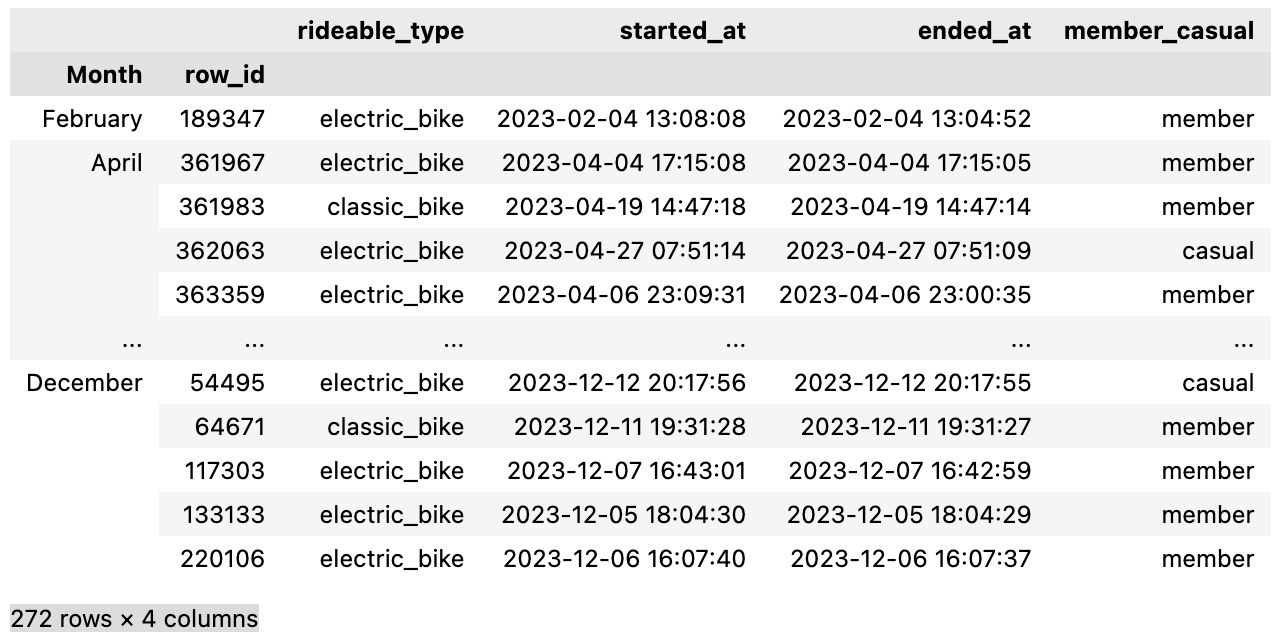
\includegraphics[scale=0.56]{imgNEG.png}
	\caption{Entries in May when the ended\_at time is before the started\_at time}
	\label{fig8}
	\end{figure}

Looking at the entries in Figure \ref{fig8}, we can see that these are cases when the \textit{ended\_at} time is before the \textit{started\_at} time by just a few seconds. It can be that in these incidents the start and end time were switched due to some glitch, perhaps the bike rental time being only a few seconds (shorter than the server response time). In the entire dataset of approximately 5.5 Million entries, there is a total of 262 entries that have this issue. Since, the dataset is large, we can simply drop these entries.


Finally, after dropping the columns related to location, and the entries with the switched times, the method \textit{count\_entries} is called once again and used to compare the cleaned dataset to the original one. The result is shown in Figure \ref{fig5}. As we can see the number of columns has changed from 13 to 4, and the number of entries is slightly less due to removing the entries where the \textit{ended\_at} time is before the \textit{started\_at} time. 
	
	\begin{figure}[h]
	\centering
	\begin{subfigure}{.4\textwidth}
	\hspace{0.5 in}
		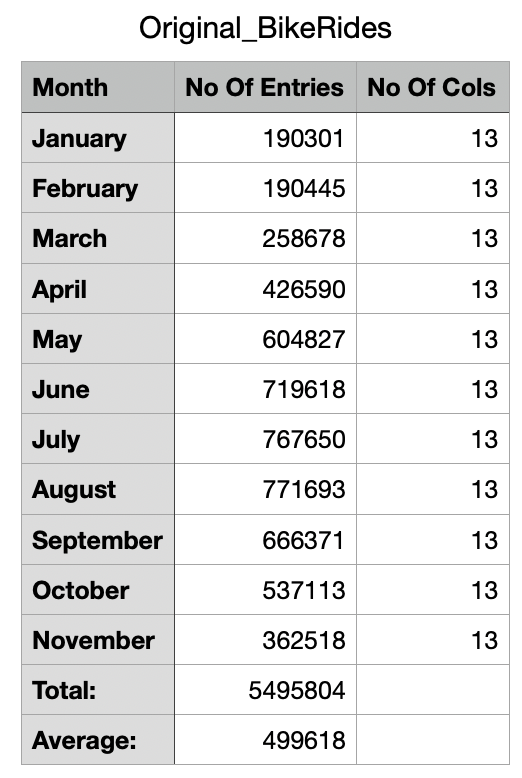
\includegraphics[scale=0.5]{img2.png}
	\end{subfigure}
	\begin{subfigure}{.4\textwidth}
	\hspace{0.5 in}
		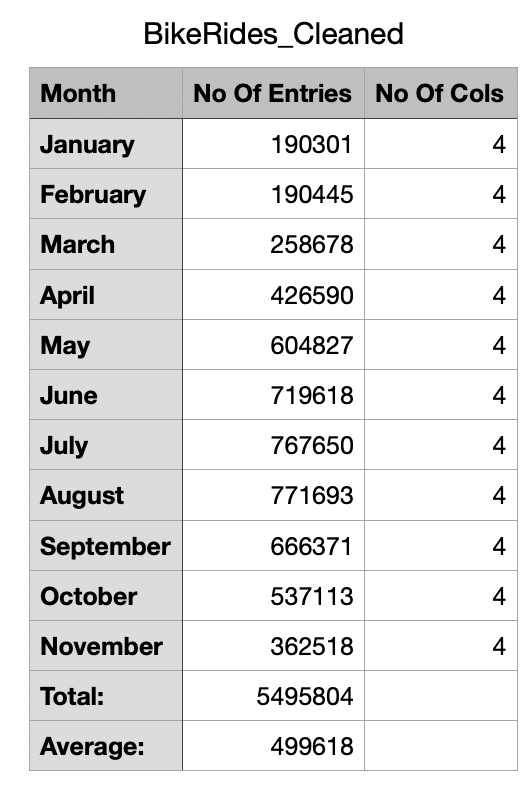
\includegraphics[scale=0.5]{img4.png}
	\end{subfigure}
	\caption{No of entries and columns before and after cleaning}
	\label{fig5}
	\end{figure}
	
	\end{itemize}

\pagebreak
	
\section*{Analysis:}
\begin{itemize}
\item \textit{prepare\_data}:\\
	The method \textit{prepare\_data} adds two new columns: \textit{ride\_length}: the difference between the columns \textit{ended\_at} and \textit{started\_at} times, and \textit{day\_of\_week}: extracted from the date in \textit{started\_at}. 
	
\item \textit{statistics}:\\	
	The method \textit{statistics} calculates for each month the average and maximum ride length, as well as the mode of the day of the week; i.e. the day of the week that occurred the most. The results are shown in Figure \ref{fig9}. The mean ride length varies between 13 - 22 minutes across the months, whereas the maximum ride length is 68 days. 
	
	\begin{figure}[h]
	\centering
	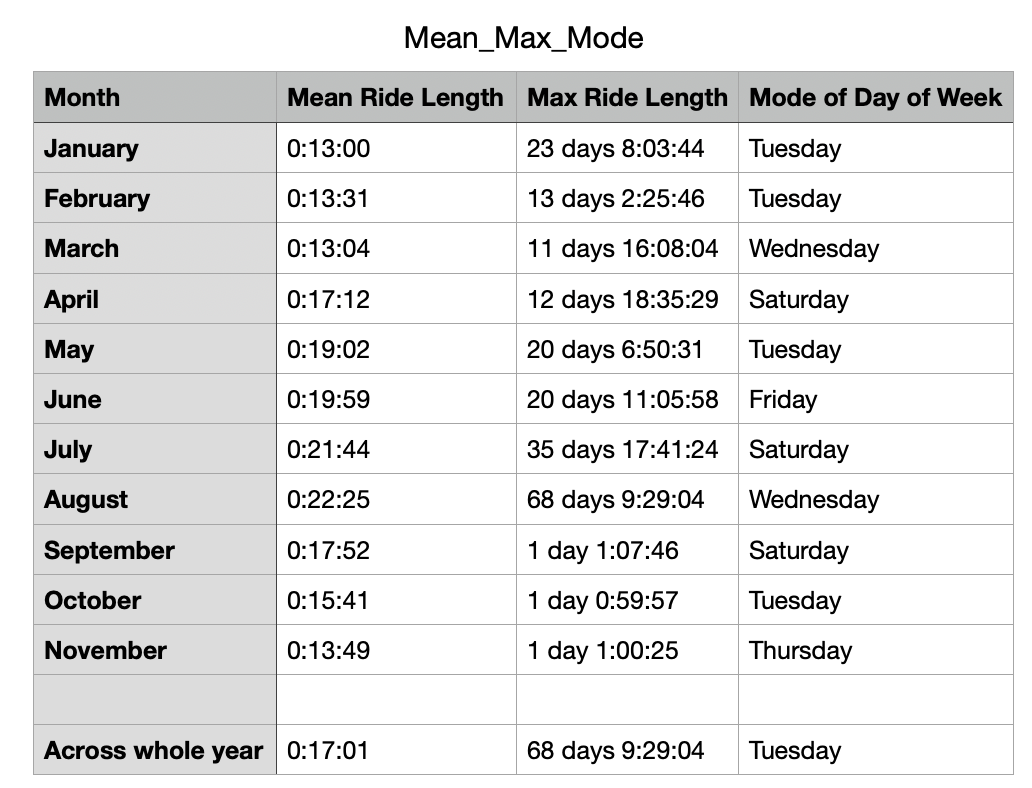
\includegraphics[width=4 in, height = 3.2 in]{imgMeanMax1.png}
	\caption{The mean and max ride length, and mode of day of the week}
	\label{fig9}
	\end{figure}
	
	\begin{figure}[h]
	\centering
	%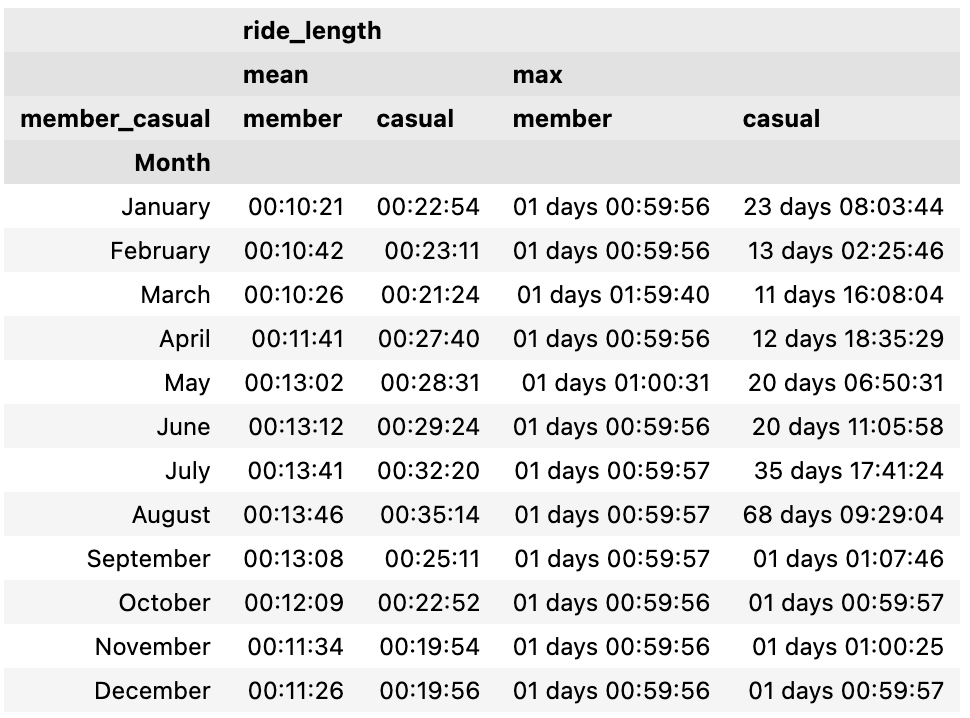
\includegraphics[width=4 in, height = 3.2 in]{imgMeanMax2.png}
	\caption{The mean and max ride length, and mode of day of the week for members and casual riders separately}
	\label{fig10}
	\end{figure}
	
\end{itemize}

\end{document}